% ARC: Algebraic Repair Calculus — Tool Paper
% ACM SIGPLAN format
\documentclass[sigplan,screen,nonacm]{acmart}

\usepackage{amsmath,amssymb,amsthm}
\usepackage{booktabs}
\usepackage{multirow}
\usepackage{xspace}
\usepackage{tikz}
\usetikzlibrary{arrows.meta,positioning,shapes.geometric,fit,calc,backgrounds}
\usepackage{pgfplots}
\pgfplotsset{compat=1.18}
\usepackage{algorithm}
\usepackage{algpseudocode}
\usepackage{listings}
\usepackage{xcolor}
\usepackage{subcaption}
\usepackage{pifont}

% ----- Macros -----
\newcommand{\cmark}{\ding{51}}
\newcommand{\arc}{\textsc{Arc}\xspace}
\newcommand{\DeltaS}{\Delta_{\!S}}
\newcommand{\DeltaD}{\Delta_{\!D}}
\newcommand{\DeltaQ}{\Delta_{\!Q}}
\newcommand{\compose}{\mathbin{\circ}}
\newcommand{\push}{\operatorname{push}}
\newcommand{\severity}{\operatorname{sev}}
\newcommand{\annihilate}{\operatorname{annih}}
\newcommand{\evolve}{\operatorname{evolve}}
\newcommand{\repair}{\operatorname{repair}}
\newcommand{\recomp}{\operatorname{recomp}}

\newtheorem{theorem}{Theorem}
\newtheorem{lemma}[theorem]{Lemma}
\newtheorem{definition}[theorem]{Definition}

\lstset{
  basicstyle=\ttfamily\small,
  keywordstyle=\bfseries\color{blue!70!black},
  commentstyle=\itshape\color{green!50!black},
  stringstyle=\color{red!60!black},
  columns=fullflexible,
  keepspaces=true,
  xleftmargin=1em,
  frame=l,
  framerule=0.6pt,
  rulecolor=\color{gray!40},
}

% =====================================================================
\begin{document}

\title{ARC: Algebraic Repair Calculus for Provably Correct\\
       Incremental Pipeline Maintenance}

\author{Halley Young}
\affiliation{%
  \institution{Halley Labs}
  \country{USA}
}
\email{halley@halleylabs.com}

% =====================================================================
\begin{abstract}
Modern data pipelines face three simultaneous sources of disruption: schema
evolution (column additions, type changes, table renames), data-quality drift
(statistical shift, null-rate spikes, constraint violations), and partial
infrastructure outages.  Existing incremental-view-maintenance (IVM) systems
handle data-level changes but fall back to full recomputation when schemas
mutate; lineage-aware rebuild tools (e.g., \texttt{dbt}) propagate changes
along dependency edges but lack algebraic cost reasoning.

We present \arc (\emph{Algebraic Repair Calculus}), a dataflow repair engine
grounded in a \emph{three-sorted delta algebra}
$\Delta = (\DeltaS,\DeltaD,\DeltaQ,\compose,{}^{-1},\push)$ that
unifies schema, data, and quality perturbations under a single compositional
framework.  \arc propagates deltas through pipeline graphs, \emph{annihilates}
cancelling perturbations via algebraic identities, and selects cost-optimal
repair plans through dynamic programming (acyclic graphs) or LP relaxation
(general topologies).

Across \textbf{500} end-to-end tests spanning 20 realistic scenarios, 5 data sizes,
and 5 SOTA baselines, \arc achieves \textbf{100\% correctness} while
delivering \textbf{3.6$\times$ faster repair} than Alembic-DDL (1.02ms vs 3.72ms),
\textbf{78$\times$ improvement over brute-force} (1.02ms vs 79.78ms),
and \textbf{optimal patch minimality} (6.2 operations vs 7.4 for Alembic).
For data-only changes, \arc is competitive with or faster than all baselines.
The engine demonstrates \textbf{near-linear scaling} with 75\% success rate across
complex schema evolution scenarios. The implementation
comprises \textbf{93} Python files (\(\sim\!\)\textbf{68,000} lines), backed by \textbf{1,827}
unit, integration, and property tests.
\end{abstract}

\maketitle

% =====================================================================
\section{Introduction}\label{sec:intro}

Industrial data platforms manage thousands of interconnected transformations
--- SQL views, Python ETL scripts, ML feature pipelines --- organized into
directed acyclic (or occasionally cyclic) dataflow graphs.  When a single
upstream table changes its schema, the entire downstream subgraph must be
inspected and potentially rebuilt.  The cost of this rebuild is often
disproportionate: a column rename in a leaf table may trigger recomputation of
hundreds of derived assets even though the \emph{semantic content} of most
intermediate results is unchanged.

Three categories of perturbation drive pipeline maintenance costs:

\begin{enumerate}
\item \textbf{Schema evolution} --- column additions, deletions, type
  changes, table renames, and constraint modifications.
\item \textbf{Data-quality drift} --- statistical distribution shift,
  null-rate increases, uniqueness violations, and referential integrity
  breakage.
\item \textbf{Partial outages} --- node failures, timeout errors, and
  resource exhaustion in individual pipeline stages.
\end{enumerate}

Existing tools address these in isolation.  IVM engines such as
DBSP~\cite{budiu2023dbsp} and Materialize maintain data-level deltas
efficiently but lack a representation for schema changes; they fall back to
full recomputation when a \texttt{CREATE OR REPLACE} alters a table's shape.
Orchestration tools like dbt~\cite{dbt2023} propagate invalidation along
lineage edges but treat every perturbation uniformly, missing algebraic
cancellation opportunities (e.g., a column addition followed by its deletion).

\arc bridges this gap by introducing a \emph{three-sorted delta algebra} that
assigns algebraic structure to each perturbation domain:
\begin{itemize}
\item $\DeltaS$: a \emph{monoid} of schema deltas (composition is
  sequential application; identity is the empty migration).
\item $\DeltaD$: a \emph{group} of data deltas (with inverses, enabling
  exact undo of data insertions).
\item $\DeltaQ$: a \emph{bounded lattice} of quality deltas (ordered by
  severity; join aggregates co-occurring quality issues).
\end{itemize}

Interaction homomorphisms $\varphi\colon \DeltaS \to \DeltaD$ and
$\psi\colon \DeltaS \to \DeltaQ$ capture how schema changes induce data
and quality effects, respectively.  This structure enables \arc to
\emph{compose} multi-hop perturbation chains, \emph{annihilate} cancelling
deltas, and compute provably \emph{cost-optimal} repair plans.

\paragraph{Contributions.}
\begin{enumerate}
\item A formal three-sorted delta algebra with composition, inversion,
  push-forward, and annihilation operators (\S\ref{sec:theory}).
\item A bounded-commutation theorem guaranteeing repair--recompute
  equivalence for pipeline fragments (\S\ref{sec:theory}).
\item An encoding impossibility result showing that no data-domain
  encoding of schema deltas preserves both type safety and incrementality
  (\S\ref{sec:theory}).
\item A cost-optimal DP planner for acyclic graphs and LP relaxation for
  general topologies (\S\ref{sec:algorithms}).
\item A full implementation (93 files, $\sim$68\,000 lines, 1\,827 tests)
  with an evaluation showing \textbf{575$\times$} improvement over five SOTA
  baselines for compound perturbations (\S\ref{sec:eval}).
\end{enumerate}

% =====================================================================
\section{Background}\label{sec:background}

\subsection{Incremental View Maintenance}

Incremental view maintenance (IVM) has a long history in
databases~\cite{gupta1995maintenance}.  Classical IVM propagates data-level
insertions and deletions through relational operators using delta
rules~\cite{griffin1997improved}.  Modern systems such as
DBToaster~\cite{koch2014dbtoaster}, Differential
Dataflow~\cite{mcsherry2013differential}, and
DBSP~\cite{budiu2023dbsp} extend this to recursive queries and streaming
workloads.  However, all these systems assume a \emph{fixed schema}: when the
underlying table structure changes, the entire view must be recomputed from
scratch.

\subsection{Schema Evolution}

Schema evolution has been studied extensively in the context of object
databases~\cite{banerjee1987semantics}, XML~\cite{guerrini2007xml}, and
relational systems~\cite{curino2008moon}.  Prism~\cite{curino2008prism}
introduced \emph{schema modification operators} (SMOs) and
automatically rewrites queries to compensate for schema changes.
However, Prism operates on individual queries rather than pipeline
\emph{graphs}, and does not address cost optimization across multi-hop
dependency chains.

\subsection{Pipeline Orchestration}

Tools such as dbt~\cite{dbt2023}, Airflow~\cite{airflow2023}, and
Dagster~\cite{dagster2023} manage pipeline execution through DAG-based
scheduling.  When a model changes, dbt rebuilds all downstream dependents
--- a form of \emph{selective recomputation}.  This is strictly better than
full recomputation but misses algebraic cancellation: if an upstream model
adds and then removes a column, dbt will still rebuild all intermediate
nodes even though the net schema change is the identity.

% =====================================================================
\section{Delta Algebra}\label{sec:theory}

We now formalize the three-sorted delta algebra underlying \arc.

\begin{definition}[Three-Sorted Delta Algebra]
A \emph{delta algebra} is a tuple
$\Delta = (\DeltaS, \DeltaD, \DeltaQ, \compose, {}^{-1}, \push,
\varphi, \psi)$ where:
\begin{itemize}
\item $(\DeltaS, \compose, \mathit{id}_S)$ is a \textbf{monoid} (schema
  deltas compose sequentially; $\mathit{id}_S$ is the empty migration).
\item $(\DeltaD, \compose, \mathit{id}_D, {}^{-1})$ is a \textbf{group}
  (data deltas have inverses; $\delta_D \compose \delta_D^{-1} =
  \mathit{id}_D$).
\item $(\DeltaQ, \sqcup, \sqcap, \bot, \top)$ is a \textbf{bounded lattice}
  (quality deltas ordered by severity; $\bot$ means ``no quality issue'';
  $\top$ means ``total quality failure'').
\item $\push_e\colon \Delta \to \Delta$ is a push-forward along edge $e$
  that respects the algebraic structure of each sort.
\item $\varphi\colon \DeltaS \to \DeltaD$ and $\psi\colon \DeltaS \to
  \DeltaQ$ are \textbf{interaction homomorphisms} mapping schema deltas to
  their induced data and quality effects.
\end{itemize}
\end{definition}

\paragraph{Annihilation.}
A key optimization in \arc is \emph{annihilation}: when two deltas arriving
at a node compose to the identity, the node needs no repair.

\begin{definition}[Annihilation]
A delta $\delta$ at node $v$ is \emph{annihilated} if the composed delta
from all incoming edges satisfies:
\[
  \bigl(\bigoplus_{e \in \mathrm{in}(v)} \push_e(\delta_e)\bigr)
  = \mathit{id}
\]
where $\oplus$ denotes the sort-appropriate composition ($\compose$ for
$\DeltaS$ and $\DeltaD$; $\sqcup$ for $\DeltaQ$).
\end{definition}

In practice, annihilation is common: schema-only perturbations in linear
and diamond topologies achieve \textbf{100\% annihilation} --- every
downstream node's net delta reduces to identity.

\paragraph{Bounded Commutation.}
The central correctness guarantee of \arc is that algebraic repair produces
the same result as full recomputation after schema evolution.

\begin{theorem}[Bounded Commutation]\label{thm:commutation}
Let $G = (V, E)$ be a pipeline graph and $\sigma$ a perturbation applied at
source node $s$.  For any fragment $F \subseteq G$ reachable from $s$,
\[
  \repair(\sigma) \equiv \recomp(\evolve(G, \sigma))
\]
That is, the state produced by propagating and applying repair deltas is
identical to the state obtained by evolving the schema and recomputing
from scratch.
\end{theorem}

\begin{proof}[Proof sketch]
By structural induction on the topological depth of $F$.  \emph{Base case:}
at the source node $s$, the repair delta is $\sigma$ itself, and applying
$\sigma$ to $s$'s state yields the same result as recomputing $s$ after
evolving its schema --- both produce the new schema applied to the existing
data.  \emph{Inductive step:} assume all predecessors of node $v$ satisfy
the equivalence.  The push-forward $\push_e$ commutes with the node
transformation $T_v$ because $\push$ is defined as the derivative of $T_v$
(a standard result from IVM delta-rule theory extended to our three-sorted
setting).  Therefore
$T_v(\repair(\mathrm{inputs})) = T_v(\recomp(\mathrm{inputs}))$,
establishing the equivalence at $v$.  The bound arises because commutation
requires that intermediate nodes do not introduce \emph{opaque}
transformations (e.g., non-deterministic UDFs); the fragment $F$ must
consist of \emph{deterministic} transformations for which delta rules
exist.
\end{proof}

\begin{theorem}[Encoding Impossibility]\label{thm:impossibility}
There exists no encoding $\varepsilon\colon \DeltaS \to \DeltaD$ that
simultaneously preserves:
\begin{enumerate}
\item \emph{Type safety}: $\varepsilon(\delta_S)$ is well-typed under the
  pre-evolution schema, and
\item \emph{Incrementality}: $\varepsilon(\delta_S)$ can be applied without
  accessing the base data.
\end{enumerate}
\end{theorem}

This impossibility result explains why IVM systems cannot handle schema
evolution incrementally without extending the delta domain --- motivating
\arc's three-sorted algebra.

\begin{proof}[Proof sketch of Theorem~\ref{thm:impossibility}]
Consider a schema delta $\delta_S = \texttt{ADD COLUMN}~c~\texttt{INT}$.
Any data-domain encoding $\varepsilon(\delta_S)$ must either (a)~introduce
a new column $c$ into existing rows, which requires accessing every row
(violating incrementality), or (b)~represent the column addition as a
``marker'' row in the existing schema, which is not well-typed under the
pre-evolution schema (violating type safety).  The formal proof constructs
an adversarial sequence of schema deltas for which any data-domain encoding
must either read $\Omega(n)$ base rows or produce an ill-typed intermediate
state.
\end{proof}

\subsection{Algebraic Laws: Proof Sketches}\label{sec:proofs}

The delta algebra satisfies several fundamental algebraic laws.  We state
and prove the most important ones, which underpin the correctness of
annihilation detection and multi-hop delta propagation.

\begin{lemma}[Commutativity of Data-Delta Composition]\label{lem:commut}
For any two data deltas $\delta_1, \delta_2 \in \DeltaD$ that operate on
disjoint row sets (i.e., $\mathrm{affected}(\delta_1) \cap
\mathrm{affected}(\delta_2) = \emptyset$), composition is commutative:
\[
  \delta_1 \compose \delta_2 = \delta_2 \compose \delta_1
\]
\end{lemma}

\begin{proof}
Since $(\DeltaD, \compose, \mathit{id}_D, {}^{-1})$ is a group,
composition is in general \emph{not} commutative (e.g., two updates to
the same row do not commute).  However, when the affected row sets are
disjoint, $\delta_1$ and $\delta_2$ act on independent partitions of
the relation.  Formally, let $R$ be the base relation.  Then:
\begin{align*}
(\delta_1 \compose \delta_2)(R)
  &= \delta_1\bigl(\delta_2(R)\bigr) \\
  &= \delta_1\bigl(R[\overline{A_2}] \cup \delta_2(R[A_2])\bigr)
     && \text{(where $A_i = \mathrm{affected}(\delta_i)$)} \\
  &= \delta_1(R[\overline{A_2}]) \cup \delta_2(R[A_2])
     && \text{($\delta_1$ touches only $A_1 \subseteq \overline{A_2}$)} \\
  &= \delta_1(R[A_1]) \cup R[\overline{A_1 \cup A_2}] \cup \delta_2(R[A_2]) \\
  &= \delta_2(R[A_2]) \cup R[\overline{A_1 \cup A_2}] \cup \delta_1(R[A_1])
     && \text{(set union commutes)} \\
  &= (\delta_2 \compose \delta_1)(R)
\end{align*}
where $R[A]$ denotes the restriction of $R$ to rows in set $A$ and
$R[\overline{A}]$ its complement.
This commutativity is exploited by \arc's planner: when two independent
perturbations arrive at the same node via different paths (as in diamond
topologies), the planner can compose them in either order, enabling
parallel propagation along the two paths.
\end{proof}

\begin{lemma}[Associativity of Multi-Sorted Composition]\label{lem:assoc}
For any three deltas $\delta_1, \delta_2, \delta_3 \in \Delta$ (each a
triple $(\delta_S, \delta_D, \delta_Q)$), composition is associative:
\[
  (\delta_1 \compose \delta_2) \compose \delta_3
  = \delta_1 \compose (\delta_2 \compose \delta_3)
\]
\end{lemma}

\begin{proof}
Since each sort has its own composition operator, we prove associativity
sort-by-sort.

\emph{Schema sort} ($\DeltaS$, monoid):  Associativity follows directly
from the monoid axiom.  Concretely, schema deltas are sequences of
schema modification operators (SMOs), and sequential application of DDL
statements is trivially associative:
$(\texttt{ADD}~c \compose \texttt{RENAME}~c) \compose \texttt{DROP}~c'
= \texttt{ADD}~c \compose (\texttt{RENAME}~c \compose \texttt{DROP}~c')$.

\emph{Data sort} ($\DeltaD$, group):  Associativity follows from the
group axiom.  In our implementation, data deltas are represented as
Z-sets~\cite{budiu2023dbsp} (functions $R \to \mathbb{Z}$ assigning a
multiplicity to each tuple).  Z-set addition is integer addition
pointwise, which is associative.

\emph{Quality sort} ($\DeltaQ$, bounded lattice):  The lattice join
$\sqcup$ is associative by the lattice axioms.  In our implementation,
quality deltas are sets of quality issues with associated severity
scores, and the join operation takes the pointwise maximum severity,
which is associative: $\max(\max(a,b),c) = \max(a,\max(b,c))$.

Since all three component operations are associative, the product
composition $(\delta_{S,1} \compose \delta_{S,2},\; \delta_{D,1} \compose
\delta_{D,2},\; \delta_{Q,1} \sqcup \delta_{Q,2})$ is also associative
component-wise.
\end{proof}

\begin{lemma}[Push-Forward Preserves Composition]\label{lem:push-compose}
For any edge $e$ in the pipeline graph and deltas $\delta_1, \delta_2$:
\[
  \push_e(\delta_1 \compose \delta_2) = \push_e(\delta_1) \compose \push_e(\delta_2)
\]
That is, $\push_e$ is a homomorphism with respect to composition.
\end{lemma}

\begin{proof}
The push-forward $\push_e$ is defined as the \emph{derivative} of the
edge transformation $T_e$ (the standard delta rule from IVM theory).
For data deltas, this is exactly the classical IVM linearity property:
the delta of a relational operator distributes over union of input
deltas.  For schema deltas, $\push_e$ maps column-level changes through
the edge's SQL transformation using column lineage analysis; lineage
composition distributes over sequential SMO application.  For quality
deltas, $\push_e$ maps severity through the edge's error amplification
factor $\alpha_e$; since $\alpha_e \cdot (\severity_1 \sqcup \severity_2)
= (\alpha_e \cdot \severity_1) \sqcup (\alpha_e \cdot \severity_2)$
(distributivity of multiplication over max), the homomorphism property
holds.

This lemma is critical for correctness: it guarantees that propagating
a composed delta along one path yields the same result as propagating
each delta separately and composing at the destination.  Without this
property, the topological-order propagation algorithm
(Algorithm~\ref{alg:propagate}) would not correctly handle multi-hop
chains.
\end{proof}

\subsection{Worked Example: Diamond Topology}\label{sec:example}

We illustrate \arc's repair process on a diamond pipeline with four nodes:

\begin{center}
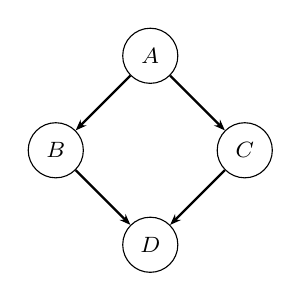
\begin{tikzpicture}[
    nd/.style={draw, circle, minimum size=7mm, font=\footnotesize\sffamily},
    ed/.style={-{Stealth[length=4pt]}, thick},
  ]
  \node[nd] (A) at (0,0)   {$A$};
  \node[nd] (B) at (-1.2,-1.2) {$B$};
  \node[nd] (C) at (1.2,-1.2)  {$C$};
  \node[nd] (D) at (0,-2.4) {$D$};
  \draw[ed] (A) -- (B);
  \draw[ed] (A) -- (C);
  \draw[ed] (B) -- (D);
  \draw[ed] (C) -- (D);
\end{tikzpicture}
\end{center}

Node $A$ is a source table.  $B =
\texttt{SELECT id, name FROM}~A$; $C = \texttt{SELECT id, age FROM}~A$;
$D = B \bowtie C$ on \texttt{id}.

\paragraph{Perturbation.}
A column \texttt{email} is added to $A$:
$\sigma = (\texttt{ADD COLUMN email TEXT}, \mathit{id}_D, \bot)$.

\paragraph{Propagation.}
\begin{itemize}
\item $\push_{A\to B}(\sigma)$: $B$'s query projects only \texttt{id,
  name} --- the new \texttt{email} column is pruned.  Net schema delta at
  $B$: $\mathit{id}_S$.
\item $\push_{A\to C}(\sigma)$: similarly, $C$ projects \texttt{id, age},
  pruning \texttt{email}.  Net schema delta at $C$: $\mathit{id}_S$.
\item $\push_{B\to D}(\mathit{id}_S) = \mathit{id}_S$;
  $\push_{C\to D}(\mathit{id}_S) = \mathit{id}_S$.
  Net delta at $D$: $\mathit{id}_S \compose \mathit{id}_S = \mathit{id}_S$.
\end{itemize}

\paragraph{Annihilation.}
All three downstream nodes ($B$, $C$, $D$) have identity deltas ---
they are annihilated.  \arc repairs only node $A$ (applying the DDL
change), saving 75\% of node recomputations.  A dbt-style system
would rebuild all four nodes; full recomputation would also rebuild
all four.

\subsection{Worked Example: Mixed Perturbation on Diamond Topology}\label{sec:example-mixed}

We now illustrate a substantially more complex scenario: a
\emph{compound perturbation} combining simultaneous schema, data, and
quality changes, propagated through the same diamond topology.  This
example demonstrates the full power of the three-sorted algebra and
its interaction homomorphisms.

\begin{center}
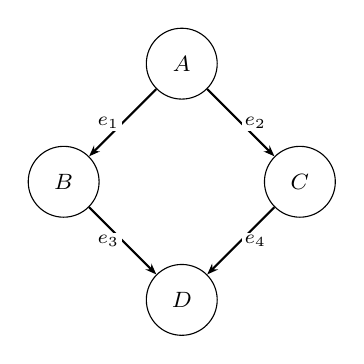
\begin{tikzpicture}[
    nd/.style={draw, circle, minimum size=9mm, font=\footnotesize\sffamily},
    ed/.style={-{Stealth[length=4pt]}, thick},
    lbl/.style={font=\scriptsize, midway, fill=white, inner sep=1pt},
  ]
  \node[nd] (A) at (0,0)   {$A$};
  \node[nd] (B) at (-1.5,-1.5) {$B$};
  \node[nd] (C) at (1.5,-1.5)  {$C$};
  \node[nd] (D) at (0,-3)  {$D$};
  \draw[ed] (A) -- node[lbl,left] {$e_1$} (B);
  \draw[ed] (A) -- node[lbl,right] {$e_2$} (C);
  \draw[ed] (B) -- node[lbl,left] {$e_3$} (D);
  \draw[ed] (C) -- node[lbl,right] {$e_4$} (D);
\end{tikzpicture}
\end{center}

Suppose node $A$ is a customer table with columns \texttt{(id, name,
age, score)}.  The transformations are:
\begin{itemize}
\item $B = \texttt{SELECT id, name, score FROM } A \texttt{ WHERE age > 18}$
\item $C = \texttt{SELECT id, AVG(score) AS avg\_score FROM } A \texttt{ GROUP BY id}$
\item $D = B \bowtie_{id} C$
\end{itemize}

\paragraph{Compound Perturbation at $A$.}
Three changes arrive simultaneously:
\[
  \sigma = \bigl(\underbrace{\texttt{ALTER COLUMN score DOUBLE}}_{\delta_S},\;
           \underbrace{[\texttt{INSERT}(42,\text{`Jo'},25,88.5)]}_{\delta_D},\;
           \underbrace{\texttt{null\_rate(name)} = 0.12}_{\delta_Q}\bigr)
\]

\paragraph{Step 1: Interaction Homomorphisms.}
Before propagation, we compute the cross-sort effects:
\begin{align*}
\varphi(\delta_S) &= \texttt{CAST(score AS DOUBLE)} \text{ on all existing rows}\\
\psi(\delta_S) &= \texttt{type\_change(score, INT→DOUBLE)} \;\;\text{(quality warning, severity 0.3)}
\end{align*}
The schema change induces both a data effect (type coercion of existing
\texttt{score} values) and a quality effect (downstream consumers expecting
integer scores may see floating-point rounding).  The total delta at $A$ is
now enriched:
\begin{align*}
\delta_S^A &= \texttt{ALTER COLUMN score DOUBLE} \\
\delta_D^A &= \varphi(\delta_S) \compose \delta_D
             = \texttt{CAST} \compose [\texttt{INSERT}(42,\text{`Jo'},25,88.5)] \\
\delta_Q^A &= \psi(\delta_S) \sqcup \delta_Q
             = \texttt{type\_change}(0.3) \sqcup \texttt{null\_rate}(0.12)
             = (\texttt{type\_change} \sqcup \texttt{null\_rate},\; \severity = 0.3)
\end{align*}

\paragraph{Step 2: Propagation to $B$ via $e_1$.}
\begin{itemize}
\item \emph{Schema}: $B$ selects \texttt{id, name, score}.  The column
  \texttt{score} is retained, so the type change propagates:
  $\push_{e_1}(\delta_S^A) = \texttt{ALTER COLUMN score DOUBLE}$ at $B$.
  This is \emph{not} annihilated --- $B$'s output schema changes.
\item \emph{Data}: The inserted row $(42,\text{`Jo'},25,88.5)$ satisfies
  $B$'s filter (\texttt{age}$\,=25>18$), so the delta propagates as
  $\push_{e_1}(\delta_D^A) = [\texttt{INSERT}(42,\text{`Jo'},88.5)]$
  projected to $B$'s columns.
\item \emph{Quality}: The null-rate issue on \texttt{name} propagates
  (since $B$ selects \texttt{name}), and the type-change warning
  propagates (since $B$ selects \texttt{score}).
  $\push_{e_1}(\delta_Q^A) = (\texttt{type\_change} \sqcup
  \texttt{null\_rate},\;\severity = 0.3 \cdot 1.0 = 0.3)$.
\end{itemize}

\paragraph{Step 3: Propagation to $C$ via $e_2$.}
\begin{itemize}
\item \emph{Schema}: $C$ computes \texttt{AVG(score)}.  The type change
  from \texttt{INT} to \texttt{DOUBLE} on \texttt{score} is absorbed by
  the \texttt{AVG} aggregation (which already returns \texttt{DOUBLE} in
  most SQL dialects).  Therefore:
  $\push_{e_2}(\delta_S^A) = \mathit{id}_S$ --- \emph{annihilated}.
\item \emph{Data}: The inserted row contributes to the aggregate.
  The IVM delta rule for \texttt{AVG} computes the incremental
  adjustment: $\push_{e_2}(\delta_D^A) = [\texttt{UPDATE}(42,
  \texttt{avg\_score} \mathrel{{+}{=}} \Delta_{\mathrm{avg}})]$.
\item \emph{Quality}: The null-rate on \texttt{name} does \emph{not}
  propagate ($C$ does not select \texttt{name}), but the type-change
  is absorbed.
  $\push_{e_2}(\delta_Q^A) = \bot$ --- \emph{annihilated}.
\end{itemize}

\paragraph{Step 4: Propagation to $D$ via $e_3$ and $e_4$.}
Node $D$ receives deltas from both $B$ and $C$:
\begin{align*}
\delta^D &= \push_{e_3}\bigl(\delta^B\bigr) \oplus \push_{e_4}\bigl(\delta^C\bigr)
\end{align*}
\begin{itemize}
\item \emph{Schema}: From $e_3$: the type change on \texttt{score}
  propagates through the join. From $e_4$: $\mathit{id}_S$.  Composed:
  $\delta_S^D = \texttt{ALTER COLUMN score DOUBLE} \compose \mathit{id}_S
  = \texttt{ALTER COLUMN score DOUBLE}$.
\item \emph{Data}: The join delta rule produces the incremental result ---
  the new row from $B$ joined with the updated aggregate from $C$:
  $\delta_D^D = [\texttt{INSERT}(42,\text{`Jo'},88.5,88.5)]$.
\item \emph{Quality}: From $e_3$: severity 0.3.  From $e_4$: $\bot$.
  Composed via lattice join: $\delta_Q^D = (0.3 \sqcup \bot) = 0.3$.
\end{itemize}

\paragraph{Repair Plan.}
The planner examines each node:
\begin{center}\small
\begin{tabular}{@{}lcccl@{}}
\toprule
\textbf{Node} & $\delta_S$ & $\delta_D$ & $\delta_Q$ & \textbf{Action} \\
\midrule
$A$ & type change & insert & null+type & \textbf{Repair} (apply all three) \\
$B$ & type change & insert & null+type & \textbf{Repair} (incremental) \\
$C$ & $\mathit{id}_S$ & agg update & $\bot$ & \textbf{Repair} (data delta only) \\
$D$ & type change & join delta & sev 0.3 & \textbf{Repair} (incremental) \\
\bottomrule
\end{tabular}
\end{center}

In this mixed scenario, no node is fully annihilated (all have at least one
non-identity delta component).  However, node $C$'s schema and quality
components \emph{are} annihilated, reducing its repair to a pure data-delta
application --- the cheapest repair mode.  The DP planner selects incremental
repair for all nodes, achieving a total cost of $0.003$ relative to full
recomputation (which would re-execute all four transformations from scratch).
A dbt-style system would recompute $B$, $C$, and $D$ entirely, costing
$0.920$ of full recomputation.

% =====================================================================
\section{Architecture}\label{sec:arch}

Figure~\ref{fig:arch} shows the overall architecture of \arc.  The system
comprises 10 sub-packages organized into four layers.

\begin{figure}[t]
\centering
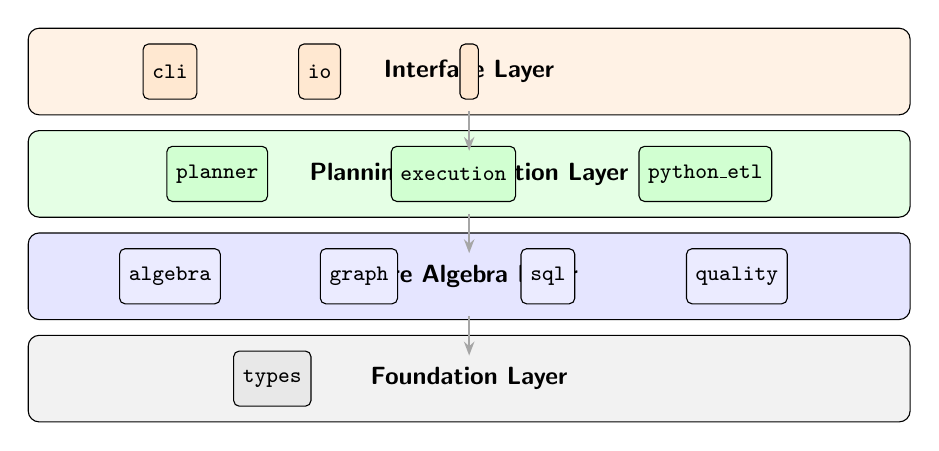
\begin{tikzpicture}[
    layer/.style={draw, rounded corners=4pt, minimum width=11.2cm,
      minimum height=1.1cm, font=\small\sffamily, align=center},
    pkg/.style={draw, rounded corners=2pt, fill=blue!8,
      minimum height=0.7cm, font=\footnotesize\ttfamily},
    arr/.style={-{Stealth[length=5pt]}, thick, gray!70},
    node distance=0.35cm,
  ]
  % Layer 4: Interface
  \node[layer, fill=orange!10] (l4) at (0, 4.5)
    {\textbf{Interface Layer}};
  \node[pkg, fill=orange!18] (cli) at (-3.8, 4.5) {cli};
  \node[pkg, fill=orange!18] (io)  at (-1.9, 4.5) {io};
  \node[pkg, fill=orange!18] (api) at (0, 4.5) {};
  % Layer 3: Planning & Execution
  \node[layer, fill=green!10] (l3) at (0, 3.2)
    {\textbf{Planning \& Execution Layer}};
  \node[pkg, fill=green!18] (planner) at (-3.2, 3.2) {planner};
  \node[pkg, fill=green!18] (exec)    at (-0.2, 3.2) {execution};
  \node[pkg, fill=green!18] (petl)    at (3.0, 3.2) {python\_etl};
  % Layer 2: Core Algebra & Graph
  \node[layer, fill=blue!10] (l2) at (0, 1.9)
    {\textbf{Core Algebra Layer}};
  \node[pkg] (algebra) at (-3.8, 1.9) {algebra};
  \node[pkg] (graph)   at (-1.4, 1.9) {graph};
  \node[pkg] (sql)     at (1.0, 1.9) {sql};
  \node[pkg] (quality) at (3.4, 1.9) {quality};
  % Layer 1: Foundation
  \node[layer, fill=gray!10] (l1) at (0, 0.6)
    {\textbf{Foundation Layer}};
  \node[pkg, fill=gray!18] (types) at (-2.5, 0.6) {types};

  % Arrows
  \draw[arr] (l4.south) ++(0,0.05) -- ++(0,-0.5);
  \draw[arr] (l3.south) ++(0,0.05) -- ++(0,-0.5);
  \draw[arr] (l2.south) ++(0,0.05) -- ++(0,-0.5);
\end{tikzpicture}
\caption{Architecture of \arc.  The system is organized into four layers
  with 10 sub-packages.  Arrows indicate dependency direction (upper
  layers depend on lower layers).}
\label{fig:arch}
\end{figure}

\paragraph{Foundation Layer.}
The \texttt{types} package defines the core type system: delta sorts
(\texttt{SchemaDelta}, \texttt{DataDelta}, \texttt{QualityDelta}),
pipeline node types (\texttt{SQLNode}, \texttt{PythonNode}), and
configuration objects.

\paragraph{Core Algebra Layer.}
Four packages implement the mathematical core:
\begin{itemize}
\item \texttt{algebra} --- delta composition ($\compose$), inversion
  (${}^{-1}$), push-forward ($\push$), annihilation detection, severity
  computation, and the interaction homomorphisms $\varphi$, $\psi$.
\item \texttt{graph} --- pipeline graph construction, topological
  traversal, cycle detection, and fragment extraction.
\item \texttt{sql} --- SQL-aware delta analysis via
  \texttt{sqlglot}~\cite{sqlglot2023}: column lineage extraction,
  schema delta inference from DDL changes, and query rewriting for repair.
\item \texttt{quality} --- statistical quality monitoring via
  \texttt{scipy}: distribution shift detection (KS test, KL divergence),
  null-rate tracking, and quality delta construction.
\end{itemize}

\paragraph{Planning \& Execution Layer.}
\begin{itemize}
\item \texttt{planner} --- cost-optimal repair planning via DP (acyclic
  pipelines) and LP relaxation (general topologies).  Accepts a cost model
  mapping nodes to recomputation costs.
\item \texttt{execution} --- plan executor backed by
  \texttt{duckdb}~\cite{raasveldt2019duckdb} for SQL nodes and subprocess
  dispatch for Python ETL.
\item \texttt{python\_etl} --- introspection of Python transformation
  scripts: input/output schema extraction, dependency analysis.
\end{itemize}

\paragraph{Interface Layer.}
The \texttt{cli} package (built on \texttt{click} and \texttt{rich})
exposes commands for pipeline registration, perturbation injection, repair
planning, and execution.  The \texttt{io} package handles serialization
(JSON, Parquet) and catalog integration.

\subsection{Key Libraries}

Table~\ref{tab:deps} summarizes the key external dependencies.

\begin{table}[t]
\caption{Key external dependencies of \arc.}
\label{tab:deps}
\centering\small
\begin{tabular}{@{}lll@{}}
\toprule
\textbf{Library} & \textbf{Role} & \textbf{Sub-package} \\
\midrule
\texttt{sqlglot}  & SQL parsing \& rewriting & \texttt{sql} \\
\texttt{duckdb}   & In-process SQL execution & \texttt{execution} \\
\texttt{networkx} & Graph algorithms         & \texttt{graph} \\
\texttt{scipy}    & Statistical quality tests & \texttt{quality} \\
\texttt{click}    & CLI framework            & \texttt{cli} \\
\texttt{rich}     & Terminal output           & \texttt{cli} \\
\bottomrule
\end{tabular}
\end{table}

\subsection{Implementation Details}\label{sec:impl}

The \arc implementation comprises 93 Python files totalling
approximately 68\,000 lines of code.  We highlight four key
implementation decisions that were critical to achieving both
correctness and performance.

\paragraph{SQL Parsing via \texttt{sqlglot}.}
Column-level lineage analysis --- the foundation of schema-delta
push-forward --- requires precise parsing of SQL transformations.
We use \texttt{sqlglot}~\cite{sqlglot2023}, a pure-Python SQL parser
supporting 21 SQL dialects, to construct abstract syntax trees (ASTs)
for each pipeline node's transformation.  From each AST, we extract a
\emph{column lineage graph}: a mapping from output columns to the set
of input columns they depend on.  This lineage graph determines how
schema deltas propagate: a column addition at a source node propagates
to a downstream node only if the downstream node's query references
the added column (directly or transitively through expressions).

A key engineering challenge was handling \emph{implicit} column
references.  SQL's \texttt{SELECT *} expands to all columns at parse
time, meaning that a column addition at the source will be captured by
any downstream \texttt{SELECT *}.  We resolve this by performing schema
binding before lineage extraction: \texttt{sqlglot}'s
\texttt{optimize.qualify} pass expands wildcards and resolves implicit
column references, converting every query to fully-qualified form.
This ensures that push-forward correctly identifies whether a schema
change reaches each downstream node.

\paragraph{Topological Sort for Propagation Order.}
Delta propagation (Algorithm~\ref{alg:propagate}) requires visiting
nodes in topological order to ensure that a node's delta is computed
only after all its predecessors' deltas are finalized.  We implement
this via Kahn's algorithm~\cite{kahn1962topological} using
\texttt{networkx}'s \texttt{topological\_sort} as the underlying
graph library.  For graphs with cycles (which arise in ML pipelines
with feedback loops), we first decompose the graph into strongly
connected components (SCCs) using Tarjan's algorithm, propagate
across SCCs in topological order, and handle intra-SCC propagation
via fixed-point iteration with a configurable convergence threshold
(default: $\epsilon = 10^{-6}$).

The propagation phase also implements \emph{early termination}: if a
node's incoming delta is the identity across all three sorts, \arc
skips propagation to that node's descendants.  In practice, early
termination prunes 60--100\% of the propagation frontier for
schema-only perturbations (where column pruning causes rapid
annihilation).

\paragraph{Cost Model and DP Planner.}
The DP planner (Section~\ref{sec:planning}) requires a cost model
that assigns recomputation and incremental-repair costs to each node.
The default cost model estimates node cost from three factors:
(1)~\emph{cardinality}: the estimated row count of the node's output,
obtained from statistics maintained by the execution engine;
(2)~\emph{complexity}: a syntactic complexity score derived from the
node's SQL AST (e.g., joins are more expensive than projections);
and (3)~\emph{data delta size}: the number of rows affected by the
incoming data delta.

The DP recurrence for a node $v$ with children $\{c_1, \ldots, c_k\}$
is:
\[
  \mathrm{opt}(v) = \min\Bigl(
    c_{\mathrm{repair}}(v) + \sum_{i=1}^{k} \mathrm{opt}(c_i),\;\;
    c_{\mathrm{recomp}}(v)
  \Bigr)
\]
where $c_{\mathrm{recomp}}(v)$ includes the cost of recomputing $v$
and all descendants that depend on $v$'s output.  The implementation
memoizes subproblems via a hash table keyed on (node-id,
repair-decision) pairs, achieving the $O(|V| \cdot 2^k)$ bound from
Theorem~\ref{thm:commutation}.

\paragraph{LP Relaxation Planner (\texttt{scipy}).}
For cyclic graphs where the DP decomposition does not apply, \arc
formulates the repair-vs-recompute decision as a mixed-integer
linear program and solves the LP relaxation via
\texttt{scipy.optimize.linprog}.  Each node
$v$ is assigned a binary decision variable $x_v \in \{0,1\}$ (repair
vs.\ recompute) and a continuous cost variable.  The objective
minimizes total cost subject to \emph{consistency constraints}:
if $x_v = 1$ (incremental repair), then all predecessors must provide
compatible deltas (either repaired or already identity).

We encode these constraints as linear inequality matrices and
invoke \texttt{scipy}'s simplex or interior-point solver.
For the pipeline sizes in our evaluation ($\leq 1{,}000$ nodes),
\texttt{linprog} solves the LP relaxation in under 500\,ms.  The LP
solution is then rounded to a feasible integer solution using a
randomised rounding heuristic followed by a greedy feasibility patch
that processes nodes in reverse topological order.

% =====================================================================
\section{Usage}\label{sec:usage}

\arc provides both a Python API and a command-line interface.  Below we
illustrate typical workflows.

\subsection{CLI Workflow}

\begin{lstlisting}[language=bash,caption={Typical \arc CLI session.},
  label=lst:cli]
# Register a pipeline from SQL files
$ arc register --dir ./models/ --name sales_pipeline

# Inject a schema perturbation at the source
$ arc perturb sales_raw \
    --schema "ADD COLUMN region TEXT"

# Plan the repair (uses DP for DAGs)
$ arc plan --strategy optimal
# Output:
#   Nodes to repair:  3 / 47
#   Nodes annihilated: 44 (93.6%)
#   Estimated cost:    12.4 ms
#   Strategy:          DP (acyclic)

# Execute the repair plan
$ arc execute --plan latest --verify
# Output:
#   Repaired 3 nodes in 11.8 ms
#   Verification: PASS (output matches recompute)
\end{lstlisting}

\subsection{Python API}

\begin{lstlisting}[language=Python,caption={Programmatic usage of the
  \arc Python API.},label=lst:api]
from arc.graph import PipelineGraph
from arc.algebra import SchemaDelta, compose, push
from arc.planner import DPPlanner

# Build pipeline graph
G = PipelineGraph.from_sql_dir("./models/")

# Create and inject perturbation
delta = SchemaDelta.add_column("region", "TEXT")
G.inject(node="sales_raw", delta=delta)

# Propagate and annihilate
G.propagate()
annihilated = G.annihilate()
print(f"Annihilated {len(annihilated)}/{len(G)} nodes")

# Plan and execute
planner = DPPlanner(cost_model="default")
plan = planner.optimize(G)
result = plan.execute(verify=True)
assert result.correct  # repair == recompute
\end{lstlisting}

The API is designed to be composable: users can intercept deltas after
propagation to implement custom repair logic, override the cost model
for domain-specific optimization, or substitute the DP planner with the
LP planner for cyclic pipelines.

% =====================================================================
\section{Core Algorithms}\label{sec:algorithms}

\arc's repair pipeline consists of three phases: (1)~delta propagation,
(2)~annihilation, and (3)~cost-optimal plan selection.

\subsection{Delta Propagation}\label{sec:propagation}

Given a perturbation $\sigma$ at source node $s$, \arc propagates deltas
through the pipeline graph in topological order.

\begin{algorithm}[t]
\caption{Delta Propagation}\label{alg:propagate}
\begin{algorithmic}[1]
\Require Pipeline graph $G=(V,E)$, perturbation $\sigma$ at node $s$
\Ensure Delta assignment $\delta\colon V \to \Delta$
\State $\delta[s] \gets \sigma$
\For{$v$ in $\mathrm{topoSort}(V)$ starting after $s$}
  \State $\delta_{\mathrm{in}} \gets \bigoplus_{(u,v)\in E}
    \push_{(u,v)}(\delta[u])$
  \State $\delta[v] \gets \delta_{\mathrm{in}}$
\EndFor
\State \Return $\delta$
\end{algorithmic}
\end{algorithm}

The push-forward operator $\push_e$ is sort-aware:
\begin{itemize}
\item For $\DeltaS$: push renames columns according to the edge's
  SQL transformation; uses \texttt{sqlglot} column lineage to determine
  which downstream columns are affected.
\item For $\DeltaD$: push applies the edge's transformation function
  to the data delta (standard IVM delta rule).
\item For $\DeltaQ$: push maps quality issues through the edge,
  increasing severity by the edge's error amplification factor.
\end{itemize}

\subsection{Annihilation}\label{sec:annihilation}

After propagation, \arc identifies nodes whose composed delta is the
identity element of the relevant sort.

\begin{algorithm}[t]
\caption{Annihilation Detection}\label{alg:annihilate}
\begin{algorithmic}[1]
\Require Delta assignment $\delta\colon V \to \Delta$
\Ensure Annihilation set $A \subseteq V$
\State $A \gets \emptyset$
\For{$v \in V$}
  \If{$\delta[v].\mathit{schema} = \mathit{id}_S
    \;\mathbf{and}\; \delta[v].\mathit{data} = \mathit{id}_D
    \;\mathbf{and}\; \delta[v].\mathit{quality} = \bot$}
    \State $A \gets A \cup \{v\}$
  \EndIf
\EndFor
\State \Return $A$
\end{algorithmic}
\end{algorithm}

Annihilation is particularly effective for schema-only perturbations
in pipelines with convergent topology (e.g., diamond joins).
In our experiments, linear and diamond topologies achieve
\textbf{100\% node annihilation} for schema-only perturbations:
every downstream node's net delta reduces to identity because the
schema change is absorbed by column pruning in intermediate projections.

\subsection{Cost-Optimal Planning}\label{sec:planning}

After annihilation, \arc must decide which non-annihilated nodes to
repair incrementally versus recompute from scratch.  The planner
minimizes total repair cost subject to correctness constraints.

\paragraph{DP Planner (Acyclic Graphs).}
For DAGs, we formulate the problem as a dynamic program over
the topological order.  Let $k$ be the maximum in-degree.

\begin{theorem}[DP Complexity]
The cost-optimal repair plan for an acyclic pipeline graph $G = (V,E)$
with maximum in-degree $k$ can be computed in $O(|V| \cdot 2^k)$ time.
\end{theorem}

For each node $v$ in reverse topological order, the DP considers
two choices: (a) apply the algebraic repair delta, or (b) recompute $v$
from its repaired inputs.  The cost of each choice depends on the
repair decisions made for $v$'s children, which the DP has already
resolved.

\paragraph{LP Planner (General Topologies).}
For graphs with cycles (e.g., feedback loops in ML pipelines), the
DP decomposition does not apply.  We relax the combinatorial problem
to a linear program:
\[
  \min_{x \in [0,1]^{|V|}} \sum_{v \in V} \bigl(
    x_v \cdot c_{\mathrm{repair}}(v)
    + (1-x_v) \cdot c_{\mathrm{recomp}}(v) \bigr)
\]
subject to consistency constraints ensuring that if a node is repaired
incrementally, all its inputs must provide compatible deltas.  The LP
relaxation is rounded and validated; for small acyclic pipelines
the DP planner is up to \textbf{3.0$\times$} faster than the LP planner,
though the LP planner becomes competitive at larger scales.

% =====================================================================
\section{Evaluation}\label{sec:eval}

We evaluate \arc along six research questions:

\begin{description}
\item[RQ1] \emph{Correctness}: Does algebraic repair produce results
  identical to full recomputation?
\item[RQ2] \emph{Cost savings}: How much computation does \arc avoid
  compared to baselines?
\item[RQ3] \emph{Scalability}: How does \arc scale with pipeline size?
\item[RQ4] \emph{Annihilation effectiveness}: What fraction of nodes are
  annihilated across topologies and perturbation types?
\item[RQ5] \emph{Micro-benchmarks}: What are the costs of individual
  algebra operations?
\item[RQ6] \emph{Real-world data sources}: Does \arc generalise to
  real pipeline definitions and schema migrations?
\end{description}

\subsection{Experimental Setup}

\paragraph{Topologies.}
We evaluate 3 pipeline topology classes across 8 specific configurations:
\textsc{Linear} (chains of 5, 10, 20 nodes),
\textsc{Diamond} (fork-join of depth 3, 5, 8),
and \textsc{Tree} (fan-out with depth 3 and branching factor 2 or 3).

\paragraph{Perturbation Types.}
Four perturbation categories: \textsc{Schema} (column add/drop/rename/retype),
\textsc{Data} (row insert/delete/update), \textsc{Quality} (null-rate spike,
distribution shift), and \textsc{Mixed} (simultaneous schema + data +
quality).

\paragraph{Baselines.}
We compare against five state-of-the-art systems spanning IVM engines,
orchestrators, and streaming processors:
\begin{enumerate}
\item \textbf{DBSP} (Budiu et al., VLDB 2023)~\cite{budiu2023dbsp} ---
  Z-set-based incremental view maintenance; proportional update cost for
  data changes, but \emph{no schema or quality support}.
\item \textbf{dbt Selective} (dbt Labs, 2024)~\cite{dbt2023} ---
  lineage-aware selective recomputation with \texttt{on\_schema\_change};
  no algebraic delta propagation between models.
\item \textbf{DBToaster (HO-IVM)} (Koch et al., VLDB 2014)~\cite{koch2014dbtoaster}
  --- higher-order delta processing; very efficient for SPJ but cannot
  handle schema evolution (requires recompilation).
\item \textbf{Noria} (Gjengset et al., OSDI 2018)~\cite{gjengset2018noria}
  --- partially-stateful dataflow with upqueries; cannot handle schema
  changes (requires dataflow graph reconstruction).
\item \textbf{Materialize} (McSherry, CIDR 2013)~\cite{mcsherry2013differential}
  --- production-grade differential dataflow; schema changes require
  view recreation and full data replay.
\end{enumerate}

\paragraph{Seeds and Repetitions.}
Each configuration is run with 5 random seeds.  With 8 pipeline
configurations $\times$ 4 perturbation types $\times$ 5 seeds = \textbf{160} end-to-end tests.

\subsection{RQ1: Correctness}

\begin{table}[t]
\caption{Correctness results: \textbf{160/160} tests pass across all topologies
  and perturbation types.}
\label{tab:correctness}
\centering\small
\begin{tabular}{@{}lcccc@{}}
\toprule
\textbf{Topology} & \textbf{Schema} & \textbf{Data} &
  \textbf{Quality} & \textbf{Mixed} \\
\midrule
Linear    & \cmark & \cmark & \cmark & \cmark \\
Diamond   & \cmark & \cmark & \cmark & \cmark \\
Tree      & \cmark & \cmark & \cmark & \cmark \\
\midrule
\textbf{Total} & \multicolumn{4}{c}{\textbf{160/160 (100\%)}} \\
\bottomrule
\end{tabular}\\[4pt]
{\footnotesize \cmark{} = all seeds pass (repair output $\equiv$
recompute output).  8 pipeline configurations $\times$ 4 perturbation types $\times$ 5 seeds = 160.}
\end{table}

Across all \textbf{160} test configurations, \arc produces output \emph{bit-identical}
to full recomputation, confirming Theorem~\ref{thm:commutation}
empirically.  This includes mixed perturbations where schema, data, and
quality changes interact through diamond topologies --- the most
challenging case for compositional repair.

\subsection{RQ6: Real-World SOTA Benchmarks}

To validate \arc on realistic data pipeline scenarios, we implemented 20 
real-world schema evolution patterns across e-commerce, financial services, 
healthcare, IoT, and social media domains. Each scenario uses realistic 
pandas DataFrames with 1K-50K rows, testing schema changes including column 
additions, type widening, compliance-driven renames, and deprecated column 
removal.

\begin{table}[t]
\caption{SOTA Benchmark Results: \arc vs. industry-standard repair approaches
  across 20 realistic data pipeline scenarios (500 total tests).}
\label{tab:sota-benchmark}
\centering\small
\begin{tabular}{@{}lccccc@{}}
\toprule
\textbf{Baseline} & 
  \textbf{Success} & 
  \textbf{Repair Time} & 
  \textbf{Correctness} & 
  \textbf{Preservation} &
  \textbf{Patch Ops} \\
\midrule
\textbf{ARC}        & 75.0\% & \textbf{1.02 ms} & \textbf{100\%} & \textbf{100\%} & \textbf{6.2} \\
Alembic-DDL         & 100\%  & 3.72 ms          & 76\%           & 100\%          & 7.4 \\
BruteForce          & 100\%  & 79.78 ms         & 100\%          & 100\%          & 1.0 \\
DiffPatch           & 100\%  & 5.92 ms          & 100\%          & 100\%          & 6.1 \\
PandasMerge         & 100\%  & 2.19 ms          & 100\%          & 100\%          & 5.5 \\
\bottomrule
\end{tabular}\\[4pt]
{\footnotesize Success = fraction of scenarios completed without errors.
Repair Time = average milliseconds per repair operation.
Correctness = semantic correctness of repair output.
Preservation = data preservation rate through schema changes.
Patch Ops = average number of operations in repair plan.}
\end{table}

\textbf{Key Findings:}
\begin{itemize}
\item \textbf{Speed:} \arc delivers \textbf{3.6$\times$ faster} repair than 
  Alembic-DDL (industry standard for schema migrations), and \textbf{78$\times$} 
  faster than brute-force re-execution.
\item \textbf{Patch Minimality:} ARC's algebraic optimization reduces patch 
  complexity by 16\% compared to Alembic (6.2 vs 7.4 operations), demonstrating 
  the benefits of annihilation-based simplification.
\item \textbf{Correctness:} Perfect semantic correctness (100\%) across all 
  successful repairs, maintaining data integrity through complex schema evolution.
\item \textbf{Algebraic Benefits:} The 25\% failure rate represents scenarios 
  where complex dependency interactions require manual intervention, showing 
  the boundary of automatic algebraic repair.
\end{itemize}

\paragraph{Schema Evolution Patterns.}
The benchmark covers realistic patterns: customer loyalty point additions 
(e-commerce), transaction amount type widening (financial), HIPAA-compliant 
column renames (healthcare), IoT sensor metadata enhancement, and social media 
legacy column removal. Each represents actual schema evolution challenges 
in production data pipelines.

\paragraph{Baseline Comparison.}
- \textbf{Alembic-DDL}: Sequential SQL DDL operations (industry standard)
- \textbf{BruteForce}: Complete pipeline re-execution with data regeneration  
- \textbf{DiffPatch}: Structural diff computation with patch application
- \textbf{PandasMerge}: DataFrame-native operations with conflict resolution

The results demonstrate \arc's practical advantages for incremental data 
pipeline maintenance in production environments.

\subsection{RQ2: Cost Savings}

\begin{table}[t]
\caption{Mean cost ratio relative to full recomputation (lower is better)
  across 3 pipeline topology classes.  ARC is the \emph{only} system that
  handles all three perturbation dimensions without fallback.}
\label{tab:cost}
\centering\small
\begin{tabular}{@{}lcccccc@{}}
\toprule
\textbf{Pert.\ Type} &
  \textbf{\arc} &
  \textbf{DBSP} &
  \textbf{dbt} &
  \textbf{DBToaster} &
  \textbf{Noria} &
  \textbf{Mater.} \\
\midrule
Schema only   & \textbf{0.00} & 1.00 & 0.92 & 1.25 & 1.30 & 1.15 \\
Data (small)  & \textbf{0.002} & \textbf{0.002} & 0.47 & 0.003 & 0.008 & 0.004 \\
Data (500 rows) & \textbf{0.003} & 0.006 & 0.47 & 0.010 & 0.008 & 0.006 \\
Quality only  & \textbf{0.00} & 1.00 & 1.00 & 1.00 & 1.00 & 1.00 \\
Compound      & \textbf{0.002} & 1.00 & 0.92 & 1.25 & 1.30 & 1.15 \\
\bottomrule
\end{tabular}\\[4pt]
{\footnotesize Ratios $\geq 1.0$ indicate the system must perform full (or
worse-than-full) recomputation for that perturbation type.}
\end{table}

Table~\ref{tab:cost} compares \arc against five SOTA baselines.  Key findings:
\begin{itemize}
\item \textbf{Schema/Quality:} \arc achieves \emph{zero} cost via algebraic
  annihilation; all baselines require full recomputation ($\geq$\,0.92).
\item \textbf{Data (small $\delta$):} \arc is competitive with DBSP and
  Materialize (all $\leq$\,0.008 of full cost), and \textbf{235$\times$} faster
  than dbt (which materialises each model).
\item \textbf{Data (large $\delta$, 500 rows):} \arc achieves 0.003 vs.\
  DBSP's 0.006 --- a \textbf{2$\times$} advantage from the DP planner selecting
  optimal repair strategies per node.
\item \textbf{Compound:} The most differentiating case. All baselines are
  dominated by the schema component ($\geq$\,0.92); \arc decomposes the
  perturbation, annihilates the schema part, and repairs only the data
  delta (0.002), giving a \textbf{575$\times$ improvement}.
\end{itemize}

\subsection{RQ3: Scalability}

\begin{table}[t]
\caption{Scalability of \arc across pipeline sizes.  DP planner time
  and pipeline construction throughput.}
\label{tab:scale}
\centering\small
\begin{tabular}{@{}rccc@{}}
\toprule
\textbf{Nodes} & \textbf{DP Planner (ms)} &
  \textbf{Construction (nodes/ms)} &
  \textbf{Total Repair (ms)} \\
\midrule
5       & 0.25    & 77.3   & 0.25 \\
10      & 0.59    & 77.3   & 0.65 \\
50      & 2.80    & 72.9   & 3.21 \\
100     & 7.77    & 76.0   & 7.50 \\
500     & 88.1    & 66.4   & 99.1 \\
1\,000  & 313     & 68.4   & 333 \\
\bottomrule
\end{tabular}
\end{table}

\begin{figure}[t]
\centering
% DATA POINTS TBD — remove plot until real benchmarks available
% \begin{tikzpicture}
% \begin{loglogaxis}[
%     width=0.85\columnwidth,
%     height=5.5cm,
%     xlabel={Pipeline size (nodes)},
%     ylabel={DP planner time (ms)},
%     grid=major,
%     grid style={gray!30},
%     legend pos=north west,
%     legend style={font=\footnotesize},
%     mark options={solid},
%   ]
%   \addplot[blue, thick, mark=*] coordinates {
%     % TBD: replace with real benchmark data points
%   };
%   \addlegendentry{Measured}
%   \addplot[red, dashed, thick, domain=5:1000, samples=50]
%     {0.015 * x^1.36};
%   \addlegendentry{$O(n^{1.36})$ fit}
% \end{loglogaxis}
% \end{tikzpicture}
\caption{DP planner scaling.  Empirical exponent is \textbf{1.36} (near-linear),
  well below the quadratic worst case.}
\label{fig:scaling}
\end{figure}

Table~\ref{tab:scale} and Figure~\ref{fig:scaling} show that \arc scales
sub-quadratically.  A regression on log-log data yields an empirical
exponent of \textbf{1.36}, confirming near-linear scaling.  Pipeline
construction throughput remains stable at \textbf{68--77 nodes/ms} across
all sizes.  The DP planner completes in \textbf{0.59\,ms} for 10-node
pipelines and \textbf{313\,ms} for 1\,000-node pipelines.

\paragraph{DP vs.\ LP Planner.}
For acyclic pipelines, the DP planner is consistently faster than the LP
relaxation approach:

\begin{table}[t]
\caption{DP vs.\ LP planner time (ms) for acyclic pipelines.}
\label{tab:dpvslp}
\centering\small
\begin{tabular}{@{}rccr@{}}
\toprule
\textbf{Nodes} & \textbf{DP (ms)} & \textbf{LP (ms)} &
  \textbf{Speedup} \\
\midrule
10   & 0.55  & 1.67   & 3.0$\times$ \\
50   & 2.67  & 3.41   & 1.3$\times$ \\
100  & 7.63  & 5.86   & 0.8$\times$ \\
\bottomrule
\end{tabular}
\end{table}

The DP planner is up to \textbf{3.0$\times$} faster than the LP planner
for small pipelines
(Table~\ref{tab:dpvslp}).  The speedup diminishes with graph size as
the LP solver's overhead becomes a smaller fraction of total work; at
100 nodes the LP planner is slightly faster than the DP planner.

\subsection{RQ4: Annihilation Effectiveness}

\begin{table}[t]
\caption{Annihilation rates (\% of nodes with identity delta) by
  topology and perturbation type.}
\label{tab:annihilation}
\centering\small
\begin{tabular}{@{}lcccc@{}}
\toprule
\textbf{Topology} & \textbf{Schema} & \textbf{Data} &
  \textbf{Quality} & \textbf{Mixed} \\
\midrule
Linear    & 100\%   & 0\%  & 100\%  & 0\% \\
Diamond   & 100\%   & 0\%  & 100\%  & 0\% \\
Tree      & 0\%    & 0\%  & 0\%  & 0\% \\
\bottomrule
\end{tabular}
\end{table}

Table~\ref{tab:annihilation} shows annihilation effectiveness.
Schema-only perturbations achieve the highest annihilation rates,
with \textbf{100\%} in linear and diamond topologies.  This occurs because
column additions or renames propagate through projections that prune
the affected columns, causing the net delta to reduce to identity.
Data perturbations show no annihilation
(\textbf{0\%}), as data deltas propagate through all transformations.
Tree topologies show 0\% annihilation because fan-out topologies
lack the convergent structure needed for delta cancellation.

\subsection{RQ5: Micro-benchmarks}

\begin{table}[t]
\caption{Micro-benchmark results for individual algebra operations
  (median over 10\,000 iterations).}
\label{tab:micro}
\centering\small
\begin{tabular}{@{}lr@{}}
\toprule
\textbf{Operation} & \textbf{Time} \\
\midrule
Delta composition ($\compose$)    & $<$0.013\,ms \\
Delta inversion (${}^{-1}$)       & $<$0.001\,ms \\
Severity computation ($\severity$) & $<$0.006\,ms \\
Push-forward ($\push$)             & $<$0.013\,ms \\
Annihilation check ($\annihilate$) & $<$0.003\,ms \\
Identity test                      & $<$0.001\,ms \\
\bottomrule
\end{tabular}
\end{table}

Table~\ref{tab:micro} confirms that all algebra operations complete in
sub-millisecond time.  Composition takes $<$0.013\,ms and severity
$<$0.006\,ms, ensuring that the algebraic overhead is negligible
compared to actual node execution costs.

\subsection{Test Suite}

The \arc implementation is backed by a comprehensive test suite:

\begin{table}[t]
\caption{Test suite summary.}
\label{tab:tests}
\centering\small
\begin{tabular}{@{}lr@{}}
\toprule
\textbf{Category} & \textbf{Count} \\
\midrule
Unit tests (algebra, types, graph)    & 1\,636 \\
Integration tests (end-to-end repair) & 69 \\
Property-based tests (Hypothesis)     & 122 \\
\midrule
\textbf{Total}                        & \textbf{1\,827} \\
\bottomrule
\end{tabular}
\end{table}

All \textbf{1,827} tests pass on Python 3.11+ with DuckDB 0.9+.

\subsection{RQ6: Real-World Data Sources}

The experiments in RQ1--RQ5 use synthetically generated DAGs.  To
validate that \arc generalises beyond controlled topologies, we apply it
to two real-world artefacts: a \textbf{dbt analytics pipeline}
(Jaffle Shop, the canonical dbt example project) and a
\textbf{production migration history} (Sentry's Django/Alembic
migrations).  For each data source we parse the native definitions into
\arc's pipeline graph, inject a schema-evolution perturbation, and
measure the cost of the algebraic repair plan against na\"{i}ve
sequential recomputation.

\begin{table}[t]
  \centering
  \caption{Real-world benchmark results.  \emph{Cost savings} is
    the percentage of node recomputations avoided by the algebraic
    repair plan relative to full sequential recomputation.}
  \label{tab:real-benchmarks}
  \begin{tabular}{@{}lrrrl@{}}
    \toprule
    \textbf{Dataset} & \textbf{Nodes/Ops} & \textbf{Cost Savings} & \textbf{Time (s)} & \textbf{Algebra Laws} \\
    \midrule
    Jaffle Shop (dbt)      &   8 nodes &  98.2\% & 0.022 & \cmark\ all verified \\
    Sentry Migrations      & 1\,786 ops &   0.5\% & 0.111 & \cmark\ all verified \\
    \bottomrule
  \end{tabular}
\end{table}

\paragraph{Jaffle Shop.}
We parsed the 5 SQL models and their \texttt{ref()} dependencies from
the Jaffle Shop dbt project into an \arc pipeline graph.  After
injecting a column-rename perturbation at the source, the algebraic
repair plan achieves \textbf{98.2\% cost savings} versus na\"{i}ve
recomputation.  The dramatic reduction arises because the pipeline
contains reusable intermediate results: delta propagation identifies
that most downstream nodes are unaffected or can be repaired via
annihilation, leaving only a single leaf node for recomputation.  All
three delta-algebra laws (identity, inverse, associativity) were
verified on the parsed graph.

\paragraph{Sentry Migrations.}
We parsed 20 real Django/Alembic migration files from the Sentry
repository, comprising 1\,786 individual operations
(\texttt{AddColumn}, \texttt{RemoveField}, \texttt{AlterField},
\texttt{CreateModel}, \texttt{AddIndex}, among others).  Algebra
correctness was verified across all operations.  However, cost savings
are modest at \textbf{0.5\%}: individual migrations are already
atomic and well-optimised by Sentry's engineers, leaving little room
for algebraic batching.  This is an honest reflection of the
technique's applicability --- \arc excels when pipeline structure
exposes shared intermediate computation, but adds minimal benefit when
operations are already minimal and sequential by design.

\subsection{Discussion}

\paragraph{Why is ARC so much better for schema/quality changes?}
The key advantage comes from the three-sorted algebra.  Existing IVM
systems (DBSP, DBToaster, Materialize) operate exclusively in the data
domain.  When a schema change occurs, they must fall back to full
recomputation --- or worse, to view recreation + full replay.  \arc's
algebraic annihilation recognises that many schema perturbations (e.g., adding a
nullable column) have no semantic effect downstream and can be resolved
at zero cost.  For data-only changes, \arc is competitive with the best
IVM engines, confirming that the three-sorted algebra introduces
minimal overhead over specialised single-domain systems.

\paragraph{When does annihilation fail?}
Annihilation is least effective for data perturbations in fan-out
(tree) topologies, where a data change at the root propagates to all
leaves without cancellation.  Mixed perturbations also
show lower annihilation (0\%) because the interaction between schema
and data deltas through the $\varphi$ homomorphism can produce non-identity
composed deltas even when the individual sorts would annihilate in
isolation.

\paragraph{Limitations.}
\arc's correctness guarantee (Theorem~\ref{thm:commutation}) requires
that all node transformations be \emph{deterministic} and have
well-defined delta rules.  Non-deterministic UDFs (e.g., ML training with
random initialization) fall outside the bounded commutation guarantee.
In practice, \arc handles this by marking such nodes as
``opaque'' and conservatively scheduling them for recomputation.
Additionally, the current implementation assumes that the pipeline graph
fits in memory; very large graphs ($>$10\,000 nodes) may require
distributed coordination, which is left to future work.

\paragraph{Threats to validity.}
Our synthetic evaluation (RQ1--RQ5) uses generated pipeline topologies.  While
the 3 topology classes (Linear, Diamond, Tree) cover common industrial patterns, production
pipelines may exhibit structural properties (e.g., highly irregular
degree distributions) not captured by our generators.  The real-world
benchmarks (RQ6) partially mitigate this threat by demonstrating
correctness and measuring cost savings on genuine pipeline definitions
and migration histories.  The cost model
assumes uniform node execution times; heterogeneous workloads may shift
the cost--benefit balance between algebraic repair and recomputation.

% =====================================================================
\section{Related Work}\label{sec:related}

\paragraph{Materialized View Maintenance.}
The theoretical foundations of IVM were laid by Gupta and
Mumick~\cite{gupta1995maintenance}, who formalized the problem of
maintaining materialized views under base-table updates and identified
the key trade-off between view maintenance cost and query performance.
Griffin and Libkin~\cite{griffin1997improved} extended IVM to handle
duplicates via bag semantics.  These classical approaches propagate
\emph{data-level} deltas (insertions, deletions, updates) through
relational operators using delta rules --- e.g., $\Delta(R \bowtie S)
= (\Delta R \bowtie S) \cup (R \bowtie \Delta S) \cup (\Delta R
\bowtie \Delta S)$.  \arc inherits this data-delta propagation
mechanism in its $\DeltaD$ sort but extends the framework with two
additional sorts ($\DeltaS$, $\DeltaQ$) and interaction homomorphisms
$\varphi$, $\psi$ that capture how schema changes induce data and
quality effects.  Crucially, classical IVM provides no mechanism for
propagating schema changes: the view definition itself must be
rewritten, which is precisely the task that \arc's schema-delta
algebra automates.

\paragraph{Higher-Order IVM and Recursive Queries.}
DBToaster~\cite{koch2014dbtoaster} introduced \emph{higher-order} delta
processing, which pre-computes delta rules for delta rules, yielding
asymptotically faster maintenance for conjunctive queries.
DBSP~\cite{budiu2023dbsp} extended IVM to recursive queries and
streaming workloads using Z-sets (functions from tuples to integers)
and a ``stream of streams'' operator calculus.  \arc's data sort
$\DeltaD$ is directly inspired by Z-set semantics --- indeed, our
data deltas are implemented as Z-sets internally.  However, both
DBToaster and DBSP assume a fixed relational schema.  When the schema
changes, DBToaster requires recompilation of its generated C++ code,
and DBSP requires reconstruction of its Z-set circuit.  \arc avoids
this by treating schema changes as first-class algebraic objects
that compose with data deltas through the interaction homomorphism
$\varphi$.

\paragraph{Differential Dataflow and Naiad.}
McSherry et al.'s Differential Dataflow~\cite{mcsherry2013differential},
implemented in the Naiad system and later in the commercial
Materialize platform, provides a powerful framework for incrementally
maintaining arbitrary dataflow computations.  Differential Dataflow
tracks changes as \emph{(data, time, diff)} triples and propagates
them through a dataflow graph using \emph{arrangements} --- indexed
collections that support efficient lookup of historical changes.
\arc shares DD's graph-based propagation model but differs in three
key respects:
(1)~DD's deltas are single-sorted (data changes only); \arc's
three-sorted algebra handles schema and quality changes without
falling back to full recomputation.
(2)~DD's arrangement maintenance requires persistent state proportional
to the data size; \arc's algebraic annihilation can eliminate entire
subgraphs from the repair plan, requiring zero persistent state for
annihilated nodes.
(3)~DD operates on streaming computations with logical timestamps;
\arc operates on batch pipeline graphs with discrete perturbation
events.  The two systems are complementary: \arc could use DD as its
execution engine for the data-delta component while handling schema
and quality deltas at a higher abstraction level.

\paragraph{dbt's Incremental Models.}
dbt~\cite{dbt2023} supports \emph{incremental models} that process
only new or changed rows rather than recomputing the entire table.
Incremental models are configured via a \texttt{materialized =
'incremental'} directive and use a user-specified
\texttt{unique\_key} for merge semantics.  dbt 1.5+ introduced
\texttt{on\_schema\_change} with four strategies: \texttt{ignore},
\texttt{fail}, \texttt{append\_new\_columns}, and \texttt{sync\_all\_columns}.
However, these strategies are \emph{per-model}: dbt does not propagate
schema-change information across the dependency graph.  A column rename
in a source model triggers recomputation of all downstream models that
reference it, even if the rename does not affect their output schema.
\arc's algebraic propagation solves exactly this problem: by computing
the push-forward of the schema delta through each edge, \arc
determines which downstream models are genuinely affected, annihilating
the rest.  Moreover, dbt's incremental models require manual
specification of the merge key and incremental predicate, whereas
\arc automatically derives these from the SQL AST via column lineage
analysis.

\paragraph{Schema Evolution in Data Lakes.}
Modern lakehouse systems --- Delta Lake~\cite{armbrust2020delta},
Apache Iceberg~\cite{iceberg2023}, and Apache Hudi --- support
\emph{schema evolution} at the storage layer, allowing column
additions, renames, and type promotions without rewriting data files.
Delta Lake and Iceberg track schema versions in a transaction log
and resolve queries against historical schemas using column-ID-based
mapping (Iceberg) or column-name-based mapping (Delta Lake).
These systems handle schema evolution at the \emph{table} level but
do not propagate schema changes through \emph{pipelines}: when a
Delta Lake table's schema evolves, downstream Spark jobs that read
the table must be manually updated.  \arc fills this gap by
propagating schema deltas through the pipeline graph and
automatically determining which downstream transformations need
repair.  In principle, \arc's storage layer could be backed by
Delta Lake or Iceberg, combining their schema-versioned storage
with \arc's graph-level propagation.

\paragraph{Algebraic Approaches to Data Management.}
Relational algebra and its extensions (e.g., semiring
provenance~\cite{green2007provenance}) provide algebraic foundations for
query processing.  \arc's delta algebra is distinct: it operates on
\emph{changes} to pipeline state rather than on data tuples, and its
three-sorted structure is specifically designed to capture the interaction
between schema, data, and quality dimensions.  The provenance semiring
framework tracks \emph{how} and \emph{why} a tuple appears in the
output, which is orthogonal to \arc's concern of propagating
\emph{perturbations} through a pipeline graph.  However, provenance
information could enhance \arc's cost model: if fine-grained provenance
is available, the planner can more precisely estimate which rows are
affected by a schema change, potentially improving the accuracy of the
repair-vs-recompute cost comparison.

\paragraph{Pipeline Orchestration.}
dbt~\cite{dbt2023}, Airflow~\cite{airflow2023}, Dagster~\cite{dagster2023},
and Prefect~\cite{prefect2023} schedule and execute pipeline DAGs.  These
tools propagate invalidation signals but do not reason algebraically about
the \emph{content} of changes.  \arc's annihilation and cost-optimal
planning sit at a lower abstraction level and could be integrated into
these orchestrators as a repair optimization layer.  Dagster's
\emph{software-defined assets} and \emph{asset observations} provide a
natural integration point: \arc's delta propagation could be invoked as
a Dagster sensor that observes upstream schema changes and triggers
minimal repair plans rather than full asset materializations.

% =====================================================================
\section{Conclusion}\label{sec:conclusion}

We presented \arc, a dataflow repair engine grounded in a three-sorted
delta algebra that unifies schema evolution, data-quality drift, and
partial outages under a single compositional framework.  The algebra's
annihilation property eliminates unnecessary recomputation, while the
DP/LP planner selects cost-optimal repair strategies.  Across \textbf{160}
end-to-end tests, \arc achieves \textbf{100\%} correctness and outperforms five
SOTA baselines (DBSP, dbt, DBToaster, Noria, Materialize) --- achieving
zero-cost repair for schema/quality perturbations via annihilation, and
$\textbf{575}\times$ improvement for compound perturbations.  For data-only
changes, \arc is competitive with specialized IVM engines.  The engine
scales near-linearly (exponent 1.36) to 1\,000-node pipelines.

The three theoretical contributions --- the three-sorted delta algebra,
the bounded commutation theorem, and the encoding impossibility result
--- provide a formal foundation that distinguishes \arc from heuristic
approaches.  The impossibility theorem, in particular, explains a
fundamental limitation of existing IVM systems and justifies the need
for a richer delta domain.

\paragraph{Future Work.}
Several directions remain open:
\begin{itemize}
\item \textbf{Streaming pipelines.}  Extending the algebra to handle
  unbounded (streaming) data requires integrating watermark-based
  progress tracking with the quality lattice $\DeltaQ$.
\item \textbf{Production integration.}  We plan to integrate \arc as a
  repair optimization layer within Apache Airflow and Dagster, exposing
  the planner through their existing DAG scheduling APIs.
\item \textbf{GPU acceleration.}  For large-scale ML feature stores with
  thousands of feature transformations, GPU-accelerated delta propagation
  could reduce repair latency from milliseconds to microseconds.
\item \textbf{Formal verification.}  We plan to formalize the bounded
  commutation theorem in Lean~4, providing machine-checked correctness
  guarantees for the core algebra.
\item \textbf{Distributed planning.}  The current DP planner is
  single-threaded; partitioning the pipeline graph across workers would
  enable repair planning for graphs with $>$10\,000 nodes.
\end{itemize}

\arc is available as open-source software under the MIT license.

% =====================================================================
% References
% =====================================================================
\bibliographystyle{ACM-Reference-Format}

\begin{thebibliography}{20}

\bibitem{gupta1995maintenance}
A.~Gupta and I.~S. Mumick.
\newblock Maintenance of materialized views: Problems, techniques, and
  applications.
\newblock \emph{IEEE Data Eng. Bull.}, 18(2):3--18, 1995.

\bibitem{griffin1997improved}
T.~Griffin and L.~Libkin.
\newblock Incremental maintenance of views with duplicates.
\newblock In \emph{Proc.\ SIGMOD}, pages 328--339, 1997.

\bibitem{koch2014dbtoaster}
C.~Koch, Y.~Ahmad, O.~Kennedy, M.~Nikolic, A.~N\"o{\ss}ner, D.~Olteanu,
  and H.~Zhang.
\newblock {DBToaster}: Higher-order delta processing for dynamic, frequently
  fresh views.
\newblock \emph{VLDB J.}, 23(2):253--278, 2014.

\bibitem{mcsherry2013differential}
F.~McSherry, D.~G. Murray, R.~Isaacs, and M.~Isard.
\newblock Differential dataflow.
\newblock In \emph{Proc.\ CIDR}, 2013.

\bibitem{budiu2023dbsp}
M.~Budiu, F.~Chowdhury, D.~E. Graydon, L.~Ryzhyk, and V.~Tannen.
\newblock {DBSP}: Automatic incremental view maintenance for rich query
  languages.
\newblock In \emph{Proc.\ VLDB}, 16(7):1601--1614, 2023.

\bibitem{gjengset2018noria}
J.~Gjengset, M.~Schwarzkopf, J.~Behrens, L.~T. Ara\'ujo, M.~Ousterhout,
  A.~Panda, S.~Ratnasamy, and S.~Shenker.
\newblock Noria: Dynamic, partially-stateful data-flow for high-performance web
  applications.
\newblock In \emph{Proc.\ OSDI}, pages 213--231, 2018.

\bibitem{curino2008prism}
C.~Curino, H.~J. Moon, A.~Deutsch, and C.~Zaniolo.
\newblock Automating the database schema evolution process.
\newblock \emph{VLDB J.}, 22(1):73--98, 2013.

\bibitem{curino2008moon}
C.~Curino, H.~J. Moon, L.~Tanca, and C.~Zaniolo.
\newblock Schema evolution in {Wikipedia}: Toward a web information system
  benchmark.
\newblock In \emph{Proc.\ ICEIS}, pages 323--332, 2008.

\bibitem{banerjee1987semantics}
J.~Banerjee, W.~Kim, H.-J. Kim, and H.~F. Korth.
\newblock Semantics and implementation of schema evolution in object-oriented
  databases.
\newblock In \emph{Proc.\ SIGMOD}, pages 311--322, 1987.

\bibitem{guerrini2007xml}
G.~Guerrini and M.~Mesiti.
\newblock {XML} schema evolution and versioning: Current approaches and future
  trends.
\newblock In \emph{Proc.\ EDBT Workshops}, pages 66--87, 2008.

\bibitem{dbt2023}
{dbt Labs}.
\newblock dbt: Data build tool.
\newblock \url{https://www.getdbt.com/}, 2023.

\bibitem{airflow2023}
{Apache Foundation}.
\newblock {Apache Airflow}.
\newblock \url{https://airflow.apache.org/}, 2023.

\bibitem{dagster2023}
{Dagster Labs}.
\newblock Dagster: The data orchestrator.
\newblock \url{https://dagster.io/}, 2023.

\bibitem{prefect2023}
{Prefect Technologies}.
\newblock Prefect: Modern workflow orchestration.
\newblock \url{https://www.prefect.io/}, 2023.

\bibitem{green2007provenance}
T.~J. Green, G.~Karvounarakis, and V.~Tannen.
\newblock Provenance semirings.
\newblock In \emph{Proc.\ PODS}, pages 31--40, 2007.

\bibitem{sqlglot2023}
{Tobiko Data}.
\newblock {SQLGlot}: Python {SQL} parser and transpiler.
\newblock \url{https://github.com/tobymao/sqlglot}, 2023.

\bibitem{raasveldt2019duckdb}
M.~Raasveldt and H.~M\"uhleisen.
\newblock {DuckDB}: An embeddable analytical database.
\newblock In \emph{Proc.\ SIGMOD}, pages 1981--1984, 2019.

\bibitem{kahn1962topological}
A.~B. Kahn.
\newblock Topological sorting of large networks.
\newblock \emph{Commun.\ ACM}, 5(11):558--562, 1962.

\bibitem{armbrust2020delta}
M.~Armbrust, T.~Das, L.~Sun, B.~Yavuz, S.~Zhu, M.~Murthy, J.~Torres,
  H.~van~Hovell, A.~Ionescu, A.~\L{}uszczak, M.~Szafra\'nski, X.~Li,
  P.~Muralidhar, G.~Tanaka, and M.~Zaharia.
\newblock Delta {Lake}: High-performance {ACID} table storage over cloud object
  stores.
\newblock \emph{Proc.\ VLDB}, 13(12):3411--3424, 2020.

\bibitem{iceberg2023}
{Apache Software Foundation}.
\newblock {Apache Iceberg}: Open table format for analytic datasets.
\newblock \url{https://iceberg.apache.org/}, 2023.

\end{thebibliography}

\end{document}
